\documentclass[%
 %reprint,
 %twocolumn,
 %superscriptaddress,
 %groupedaddress,
 %unsortedaddress,
 %runinaddress,
 %frontmatterverbose,
  preprint,
 showpacs,
 showkeys,
 preprintnumbers,
 %nofootinbib,
 %nobibnotes,
 %bibnotes,
 amsmath,amssymb,
 aps,
 %prl,
   pra,
 % prb,
 % rmp,
 %prstab,
 %prstper,
  longbibliography,
 %floatfix,
 %lengthcheck,%
 ]{revtex4-1}

%\usepackage{cdmtcs-pdf}

\usepackage[breaklinks=true,colorlinks=true,anchorcolor=blue,citecolor=blue,filecolor=blue,menucolor=blue,pagecolor=blue,urlcolor=blue,linkcolor=blue]{hyperref}
\usepackage{graphicx}% Include figure files
\usepackage{url}

\usepackage{xcolor}
\usepackage{tikz}

\newtheorem{question}{Question}
\newtheorem{conjecture}[question]{Principle}
\newtheorem{challenge}[question]{Challenge}

\begin{document}


\title{The present situation in quantum mechanics and the ontological single pure state conjecture}

%\cdmtcsauthor{Karl Svozil}
%\cdmtcsaffiliation{Vienna University of Technology}
%\cdmtcstrnumber{407}
%\cdmtcsdate{September 2011}
%\coverpage

\author{Karl Svozil}
\affiliation{Institute for Theoretical Physics, Vienna
    University of Technology, Wiedner Hauptstra\ss e 8-10/136, A-1040
    Vienna, Austria}
\affiliation{Dipartimento di Scienze Pedagogiche e Filosofiche, Universit\'a  di Cagliari,\\
 Via Is Mirrionis, 1, I-09123, Cagliari, Sardinia, Italy}
\email{svozil@tuwien.ac.at} \homepage[]{http://tph.tuwien.ac.at/~svozil}
\thanks{Contribution to the 11th Biennial  International Quantum Structure Association  (IQSA) Meeting
"Quantum Structures Cagliari 2012," 23 - 27 July - Cagliari (Italy)}

\pacs{03.65.Ta, 03.65.Ud}
\keywords{quantum  measurement theory}
%\preprint{CDMTCS preprint nr. 407/2011}

\begin{abstract}
Despite its excessive success in predicting experimental frequencies and certain single outcomes,
``our quantum mechanics'' is haunted by several conceptual and technical issues; among them
(i) the (non-)existence of measurement and the cut between observer and object in an environment globally covered by a unitary (i.e. one-to-one Laplacian deterministic) evolution;
related to the question of how many-to-one mappings could possibly ``emerge'' from one-to-one functions; and also where exactly ``randomness resides;''
(ii) what constitutes a pure quantum state;
(iii) the epistemic or ontic (non-)existence of mixed states; related to the question of how non-pure states can be ``produced'' from pure ones; as well as
(iv) the epistemic or ontic existence of pure but entangled and/or coherent states containing classically mutually exclusive states;
an issue the late Schr\"odinger has called ``quantum quagmire'' or ``jellification;''
(v) the (non-)existence of quantum value indefiniteness and its purported ``resolution'' by quantum contextuality; and finally
(vi) the claim that the best interpretation of the quantum formalism is its non-interpretation.
Many of these conceptual difficulties can be overcome by assuming that only a single pure state (context) exists;
and that the quantum evolution ``permutes'' this state (context) in its Hilbert space.
\end{abstract}

\maketitle

\tableofcontents


\section{Persistent issues}

Quite rightly quantum mechanics has been lauded as one of the most successful physical theories ever developed by human thought.
Yet at the same time non-negligible areas of its formalism, let alone its interpretation, remain conceptually fuzzy and unclear.
In this respect, the situation is not too different today than it has been almost a century ago,
when Schr\"odinger published his famous series of articles
\cite{schrodinger}
on the conceptual difficulties troubling the formal framework which he had helped to create.

Since then, several important discoveries have shed new light on the foundational issues raised by Schr\"odinger and others
about ``our new quantum mechanics'' \cite[p.~866]{born-26-1}.
Alas, in this regard, it might not be totally unjustified to draw some analogies to
the fierce -- and from a contemporary perspective rather troubled and confused --
debates of Galileo and his contemporaries \cite{Camerota-galilei} {\it de motu} (on motion).

In what follows I will thus attempt to delineate  the quantum conundrum
and suggest an improved understanding and evaluation of the situation.
Thereby I confess that I cannot claim to be correct on all, or even many, or even any, of the following topics.

I will strictly remain within the boundaries of classical Hilbert space formalism of quantum theory
as outlined by von Neumann \cite{v-neumann-49}.
The notation is adopted from Mermin's introduction to quantum computation \cite{mermin-04}.




\section{Do measurements exist?}


The late Bell sarcastically observed  \cite{bell-a} that most quantum physicists appear to be
``why bother?'ers'' \cite{dirac-noworries} neglecting the
measurement problem by considering it solved ``for all practical purposes'' (FAPP).
Yet, the associated issues are much more pressing now then ever,
as technologies \cite{zeilinger:qct,stefanov-2000} based on quantum concepts of measurement
have been applied for experiments \cite{wjswz-98},
as well as deployed for cryptanalysis and industry.
In particular, at stake is the nature of randomness emerging from such devices.


\subsection{Quantum jellification}


Already around 1935 \cite{schrodinger}, Schr\"odinger considered the {\em coherent superposition}
$\vert 0 \rangle + \vert 1 \rangle$ of classically distinct, mutually exclusive and operationally separable states
$\vert 0 \rangle$
and
$\vert 1 \rangle$,
which is a direct consequence of the linear vector space formalism,
as a serious issue.
He expressed this metaphorically by a cat in a {\em coherent superposition}
``between being dead and alive'' $\vert {\textsf D} \rangle + \vert {\textsf A} \rangle$; the latter state being somehow
``induced'' by the coherent superposition of a single two-state quantum by some unspecified but supposedly hypothetical quantum evolution
\begin{equation}
\vert 0 \rangle + \vert 1 \rangle \mapsto \vert {\textsf D} \rangle + \vert {\textsf A} \rangle
\label{2012-psqm-v2-e1}
\end{equation}
``blowing up'' the microscopic coherence into the classical domain.


In 1952, Schr\"odinger maintained  \cite[pp. 19]{schroedinger-interpretation} that, quite generally,
without measurement, quantum theorists should be troubled that, due to coherent superposition
resulting in the co-existence of classically mutually exclusive alternatives,
their ``surroundings rapidly turning into a quagmire, a sort of a featureless jelly or plasma,
all contours becoming blurred, we ourselves probably becoming jelly fish.''



\subsection{Everett and Wigner's observation of a subjective observer-object cut}

Around that time,
Everett \cite[p.~454]{everett} and shortly afterwards Wigner \cite[p.~173]{wigner:mb}
observed that,
if a ``pure'' unitary (bijective, one-to-one, reversible, Laplacian-type deterministic) quantum evolution was assumed universally,
there would be no room for any ``(wave function or) state reduction mechanism''
associated with quantum measurements.
In particular, any distinction or cut between the observer and the measurement apparatus necessarily remains epistemic, subjective and conventional
and not absolute or ontic.

Because, suppose that one has defined a cut or difference between an observed quantum and a ``quasi-classical'' measurement device,
one could, at least in principle, and
``draw a larger perimeter.'' This `` `enlarged domain'' could encompass the entire previous configuration,
{\em including} the ``observed'' quantum, the cut, and the measurement device.
If the ``pure'' quantum evolution is assumed to apply universally, such a quantized system should also undergo
a unitary (bijective, one-to-one, reversible, Laplacian-type deterministic) quantum evolution.
Indeed, there is no principle why such enlargement ``shift of cuts'' could not go on forever,
until an arbitrary large system extension (either in configuration or in terms of Hilbert spaces)
is reached.
And hence, strictly speaking and disregarding resources and complexities, due to uniform unitary,
even although it may FAPP be impossible to reconstruct quantum states after  ``measurements,''
any irreducible form of irreversibility decays into thin air.

Indeed, for Everett, any form of ``classical'' measurement apparatus seemed to have been a regression
into pre-quantum physics \cite{Levy-Leblond}.
He wanted to keep the quantum formalism ``pure''
by abolishing any form of mechanism of ``wave function collapse,''
``state reduction,''
and irreversible many-to-one evolution  \cite{Barrett-2011}.


Alas, any insistence on the pure unitary quantum formalism inevitably yields  to the conceptual issue of a massive
jellification  by \cite[pp.~17-18]{werner-62}
``allowing the superpositions to continue forever $\ldots $
there is a large superposition of states, each element of which contains the observer $\ldots$
all of the elements simultaneously coexist.''

\subsection{Formal and empirical aspects of (ir-)reversibility}

Hence, after Schr\"odinger's and Everett's observations
the discomforting issue regarding quantum jellification was even more compelling.
Let us rephrase this by asking the following
{\color{blue} \begin{question}
{If ``pure'' quantum mechanics  (without any reduction mechanism) is universally valid, and if it is governed by unitary, reversible, one-to-one evolution,
how does irreversibility arise from reversibility?}
\end{question}   }
There appear to be at least three alternatives:
(i)
either to consider
the uniqueness of our experience as an idealistic illusion \cite{stace1},
(ii)
or to postulate
that ``pure'' quantum mechanics (without any reduction mechanism) is inconsistent or at least incomplete
insofar as the uniformity of the unitary quantum evolution
cannot be accommodated with the uniqueness of the state that results from a measurement;
in this case one should come up with some sort of {\em reduction mechanism} augmenting ``pure'' unitary quantum evolution;
(iii)
or to find some grounds to believe that one can have all of this
-- jellification as well as quasi-uniqueness of the phenomenology --
within the unitary framework of the quantum evolution.

Note that a not dissimilar problem is notorious also for classical statistical mechanics, although in quantum mechanics it seems
to appear even more pressing.
It has two aspects; one formal and the other empirical.

\subsubsection{`Emergence' of many-to-one from one-to-one functions?}

The formal aspect is related to question of whether it is possible to obtain an irreversible many-to-one function
from reversible one-to-one (injective) functions.
Pointedly stated, one could pose the following
{\color{blue} \begin{question}
 How can many-to-one-ness possibly `emerge' from one-to-one-ness?
\end{question}   }

More specifically, as unitary transformations are bijections (one-to-one and onto functions),
the question is if any many-to-one function (modelling the ``state reduction''
or the ``wave function collapse'')  can be constructed from bijections.

I believe that any exact solution of the quantum measurement problem has
to come up with some kind of scenario addressing these formal questions.
I also believe that, under very mild side assumptions,
(possibly excluding infinite limits),
no formal `emergence' of many-to-one-ness  from one-to-one-ness can exist.

Indeed, consider the following very elementary proof by contradiction.
Suppose (wrongly) a hypothetical many-to-one function $h(x)=h(y)$ for $x\neq y$ exists which would somehow
`emerge' from one-to-one (injective) functions.
Any such function would have to originate from the domain of one-to-one functions such that,
for all functions $f$ of this class,  $x\neq y$ implies  $f(x)\neq f(y)$
-- or, equivalently, the contrapositive statement (provable by comparison of truth tables \cite[chapter~3]{Daepp})
$f(x) = f(y)$ implies $x = y$,  a clear contradiction with the assumption.

Indeed, any bijection on some Hilbert space ${\mathfrak H}$ is a {\em permutation} of elements of ${\mathfrak H}$.
The {\em unitary transformations} form a particular permutation group (consisting of those permutations preserving the inner product),
which is a subgroup of the {\em symmetric group}
of all permutations on ${\mathfrak H}$.
(An example for a permutation which is not included in the unitary group are
transformations which do not preserve the inner product;
for instance, $f(x)=2x$,  since $\langle x\vert y\rangle \neq  \langle f(x)\vert f(y)\rangle = 4 \langle x\vert y\rangle$.)
The group property implies that any kind of composition of group elements -- in this case unitary transformations
representing some ``pure'' quantum evolution -- cannot result in elements ``outside of'' this group.
Injections form semigroups because their inverse need not exist.


Hence, the hypothesis or believe that
irreversible measurements can be reconciled with the assumption that the
``pure'' (unitary) quantum evolution is universally valid will eventually
be identified as being what it is -- an illusory {\em red herring.}
The time when this will be acknowledged by the physics community is determined
by the subjective willingness of physicists to acknowledge
and not neglect an otherwise rather trivial fact.


\subsubsection{`Undoing' measurements}

Let us state another, more empirical,
{\color{blue} \begin{question}
Is there a principle (and not only practical or technological FAPP) limit to `undo' measurements?
\end{question}   }
I believe that there is none,
as various quantum erasure experiments seem to indicate
\citep{PhysRevD.22.879,PhysRevA.25.2208,greenberger2,Nature351,Zajonc-91,PhysRevA.45.7729,PhysRevLett.73.1223,PhysRevLett.75.3783,hkwz}.
And thus,
what one calls ``measurement,''
as well as the cut between observer and object, is purely conventional \cite{svozil-2001-convention}.

Because, as has been already argued by  Everett \cite[p.~454]{everett}, and Wigner \cite[p.~173]{wigner:mb} and alluded to earlier,
even if one has located such a {\em Cartesian cut}, and drew the line between object and measurement apparatus,
this divide is whisked away into thin air by merely considering a larger, quantized system containing both the
aforementioned  object  and measurement apparatus.

\subsection{Copying and amplification of a weak quantized signal}

Although Schr\"odinger's cat metaphor sketched by Eq.
(\ref{2012-psqm-v2-e1}) could have been perceived also as a process of {\em signal amplification,}
researchers only cared to think about quantum
{\em copying} or
{\em cloning}
in the early eighties of the last century
--
%and thus more than eighty years after Planck's desperate assumption,
%followed by Einstein's correct prediction of the photoelectric effect by quanta of light
%--
in response to an (as it turned out erroneous but stimulating)
paper %by Herbert \cite{herbert}
claiming to be able to communicate faster-than-light
if generic quantum states could be copied.
These considerations have also far reaching consequences for the quantum theory of measurement.


\subsubsection{(No-)Cloning theorem}

One could also perceive jellification of macroscopic quantized systems by
starting from microscopic coherence and attempting to copy and amplify this coherence to the macroscopic domain
(say, containing quantum copies of the order of Loschmidt's constant).
Let us start lightly and assume that we would like to somehow generate a {\em single} copy of just one quantum.
This of course does  not represent a classical measurement, because the object is on par with the ``apparatus.''

We thereby do not restrict ourselves to two-dimensional Hilbert spaces
--
referring to two mutually exclusive outcomes,
which could be interpreted as representing the classical truth values
``{\tt true}''
and
``{\tt false},''
respectively
--
but consider arbitrary finite $d$--dimensional Hilbert spaces.
After all, there is no physical reason why one should prefer two dimensions over higher dimensions; just on the contrary
-- the possibility to ``interconnect'' orthogonal bases by common legs or elements
from three dimensions onward allows proofs of theorems such as the ones by Gleason and Kochen-Specker.



So, suppose (wrongly, as we are assuming this for the sake of a proof by contradiction; cf, e.g.,
\cite[pp.~39-40]{mermin-04} )
that it is somehow possible to copy $n\le d$ arbitrary but linearly independent (partial for reasons that will become clear later) Qdits
$\vert 0 \rangle , \ldots , \vert n-1 \rangle $,
by invoking some unitary transformation
$\textsf{\textbf{U}}$ on a system composed from a ``blank'' (partial) Qdit
$\vert B \rangle $ and the (partial) Qdits, such that
$\textsf{\textbf{U}}  \vert B \rangle \vert i \rangle    = \vert i \rangle \vert i \rangle $, $i=0,\ldots , n-1$
(note that this operation is $n$-to-$n$ and thus reversible).
Linearity of the unitary transformation demands that an arbitrary superposition
$\vert \psi  \rangle = a_0\vert 0 \rangle + \cdots + a_{n-1}\vert n-1 \rangle $,
together with the blank (partial) Qdit
$\vert b \rangle $,
when subjected to the (wrongly) supposed ``copier'' $\textsf{\textbf{U}}$,
gets transformed linearly into
$\textsf{\textbf{U}}  \vert B \rangle \vert \psi \rangle    = \sum_{i=0}^{n-1} a_i \vert i \rangle \vert i \rangle $.
Alas, the actual copy of
$\vert \psi  \rangle$
is
$\vert \psi  \rangle \vert \psi  \rangle = (\vert \psi  \rangle)^2
 = \sum_{i=0}^{n-1} \sum_{j=0}^{n-1} a_i  a_j \vert i \rangle \vert j \rangle
$, which contains also interference terms
$\vert i  \rangle \vert j  \rangle$, $i\neq j$,  $i,j=0,\ldots , n-1$
which do not show up in the alleged ``copy'' $\textsf{\textbf{U}}  \vert B \rangle \vert \psi \rangle    $.
Hence, if the interference terms do not vanish, then the  ``copier'' cannot copy an arbitrary superposition of (partial) Qdits.

Note, however, that it is still conceivable for  $\textsf{\textbf{U}}$ to copy (or actually just to create) correctly [the (partial) Qdits of]
an entire arbitrarily oriented orthonormal basis
${\mathfrak B} =\{ \vert {\textsf e}_0 \rangle, \vert {\textsf e}_2 \rangle, \ldots , \vert {\textsf e}_{d-1} \rangle \}$:
Consider two arbitrary elements
$\vert {\textsf e}_i \rangle$ and $\vert {\textsf e}_j \rangle$,   $i,j=0,\ldots , d-1$ of that basis, and assume
$\textsf{\textbf{U}}  \vert B \rangle \vert {\textsf e}_i \rangle    = \vert {\textsf e}_i \rangle \vert {\textsf e}_i \rangle $
and
$\textsf{\textbf{U}}  \vert B \rangle \vert {\textsf e}_j \rangle    = \vert {\textsf e}_j \rangle \vert {\textsf e}_j \rangle $.
By taking the inner products (which are preserved by the unitary transforms),
$
 \langle {\textsf e}_j \vert \langle   B \vert     \textsf{\textbf{U}}^{(-1)}
\textsf{\textbf{U}}  \vert B \rangle \vert {\textsf e}_i \rangle
=
\left( \langle {\textsf e}_j \vert \langle   {\textsf e}_j \vert \right)
\vert {\textsf e}_i \rangle \vert {\textsf e}_i \rangle$
and thus, since
$\langle   B \vert   B \rangle =1$,
we obtain
$
\langle {\textsf e}_j \vert  {\textsf e}_i \rangle
=
(\langle {\textsf e}_j \vert  {\textsf e}_i \rangle )^2
$
which is satisfied only if either
$
\langle {\textsf e}_j \vert  {\textsf e}_i \rangle
=
0
$
--
representing {\em orthogonal} vectors
--
$\vert{\textsf e}_i\rangle
\perp
\vert{\textsf e}_j\rangle  $;
or if
$
\langle {\textsf e}_j \vert  {\textsf e}_i \rangle
=
1
$
--
representing {\em collinear} (parallel) vectors $\vert{\textsf e}_i\rangle
\parallel
\vert{\textsf e}_j\rangle  $.
This is satisfied for a maximal number of non-collinear vectors
by the orthonormal basis
${\mathfrak B}$; in this case,
$
\langle {\textsf e}_i \vert  {\textsf e}_j \rangle
=\delta_{ij}$.

By induction, this analysis can be extended to an {\em arbitrary number of copies} of the original basis
${\mathfrak B}$.
Thus, it is possible to ``copy'' an arbitrary pure state (see below) with a particular ``copier''
$\textsf{\textbf{U}}_{\mathfrak B}$
associated with that basis or state.
Any such  ``copier''
$\textsf{\textbf{U}}_{\mathfrak B}$ capable of copying an arbitrary number of copies of the basis/context/state ${\mathfrak B}$ will, however,
{\em fail for all other states or bases}  ${\mathfrak B}' \neq {\mathfrak B}$.



\subsubsection{Amplification of superpositions}

The natural question arises: what happens if an experimenter {\em insists}
on applying an  ``improper copier'' $\textsf{\textbf{U}}_{{\mathfrak B}'}$
to a basis ${\mathfrak B}$; that is, what is if there is a mismatch between the
basis or state prepared and the basis or state ``analyzed?''


This question is more relevant to Schr\"odinger's cat metaphor as the perfect copy of a huge amount of
identical coherent superpositions mentioned earlier, since the
two states $ \vert {\textsf A} \rangle$ and $\vert {\textsf D} \rangle $ of the cat being alive or dead, respectively,
have no direct interpretation as
a large number of copies
of the original 50:50 superposition  $\vert 0 \rangle + \vert 1 \rangle$
between some ``classical'' single quantum states
$\vert 0 \rangle$
and
$\vert 1 \rangle$
--
surely one could not associate a collection of ${\cal N} \gg 1$ quanta
in the superposition $\left(\vert 0 \rangle + \vert 1 \rangle \right)^{\cal N}$ with a cat!
A cat physically exists as a hugely complex combination of different quanta.



Glauber \cite{glauber,Glauber-cat-86,glauber-collected-cat}
has carefully analyzed the ``amplification'' or ``blowing up'' of states such as   $\vert 0 \rangle + \vert 1 \rangle$
by explicitly constructing an amplifier which receives its energy through coupling to field modes, representing the many degrees of freedom of a ``quasi-classical''
device.
This quantum field theoretic analysis goes beyond the scope of this review.
The  outcome is a situation in which part of the information about the original state is retained,
but the final quantum state does {\em not} contain ``more'' coherence that the initial superposition.
There are more particles present after the amplification, and surely the intensity could be made arbitrary high,
but the information extractable from the output of the amplifier cannot be increased
by amplification of the original signal.
The reason for this is the inevitable introduction of ``noise'' -- that is, additional quanta -- originating from the
field modes used by the amplification process.
The underlying process is a multipartite unitary transformation, and thus again is reversible in principle, but FAPP irreversible.




\subsection{Some FAPP attempts to get rid of jellification}

There exist various attempts to circumvent jellification from other perspectives.
One claim is about the FAPP ``destruction'' of a superposition  $\vert {\textsf D} \rangle + \vert {\textsf A} \rangle$ of macroscopic distinct states
such as $\vert {\textsf D} \rangle $ and $ \vert {\textsf A} \rangle$    because of the
``environment effectively monitoring'' such a state \cite{RevModPhys.75.715}.
Thereby, no explicit observer needs to be present, because as
Mandel concludes \cite{mandel-operational-cat},
based on an interferometer experiment \cite{zou-wang-mandel:91a,zou-wang-mandel:91b},
``the
mere feasibility of the observations, in principle, is sufficient to achieve the same effect, because
the state reflects not only what is known, but also what is knowable in principle.''
This amounts to claiming that FAPP macroscopic superpositions cannot exist.

Mandel also pointed out that any kind of amplification of a ``weak'' coherent quantum signal by a classical device
(such as a photomultiplier or avalanche photodiode) and the resulting FAPP classical currents {\it et cetera}
must necessarily render
``the possibility, in principle, of making a measurement that identifies the [classical] state
[either $\vert 0 \rangle$ or $\vert 1 \rangle$], without physically disturbing
the system,'' and thus ``the coherent superposition is lost.''

Alas these attempts to get rid of jellification can only be perceived as FAPP applicable;
in a very similar way as in classical statistical mechanics the entropy is increasing FAPP.


\subsection{Analogues in classical statistical mechanics}

Just as Newtonian physics and electromagnetism appear to be reversible,
the quantum measurement conundrum is characterized by the reversibility of
the unitary quantum evolution.
In this respect, it
bears some analogy to Loschmidt's reversibility paradox \cite[p.~139]{Loschmidt}
--
that, for large isolated systems with reversible laws of motion, FAPP  one never
observes a decrease in entropy
--
and Zermelo's recurrence objection  \cite[pp.~18ff]{Ebbinghaus-Zermelo}
--
that, as an isolated system will infinitely often approach its initial
state, its entropy will infinitely often approach the initial entropy and thus cannot constantly
increase
--
in classical statistical mechanics.


And just as in statistical mechanics, these arguments appear to apply FAPP but need not be strictly true.
Nevertheless, any kind of strictness beyond FAPPness in physics might not be perceived as operationally relevant (per definition),
as, for instance, formal limits involving infinities cannot be operationalized \cite{bridgman,gandy1}.


It seems that  Schr\"odinger's cat will FAPP remain either dead or alive, but can FAPP never be both dead and alive.
Just as the issues involving (ir-)reversibility in classical statistical physics,
jellification and Schr\"odinger's cat  might thus be with us forever in principle, but ruled out FAPP;
just as we might be able to assume that FAPP irreversible measurements exist.


\section{What constitutes a pure quantum state?}

Arguably the most fundamental property of a Hilbert space is its dimension.
For quantized systems, the (minimal) dimension required is the number of possible, mutually exclusive outcomes.
That is, in a generalized beam splitter scenario \cite{rzbb} which serves as a robust analogue of any quantized system,
whenever the number of (input and output) ports is $d$, so is the dimension of the Hilbert space modelling that beam splitter.
Operationally, in an ideal setup (no losses in the beam paths {\it et cetera}) one (and only one) detector, out of an array of $d$ detectors
(located after the output ports) clicks.

Any such system represents a maximal knowledge about a quantized system, which (ideally) is certain;
as well as a complete control of the preparation.
Here the terms ``maximal'' and ``complete'' refer to the fact that there is no operational procedure which could improve either the magnitude of definite knowledge,
or the precision of the preparation. Let us call any such maximal information about a physical system a state.

{\color{blue} \begin{conjecture}
A pure state is characterized by
the maximal information encodable into a physical system.
\end{conjecture}   }

Any array of $d$ detectors (or other equivalent detection equipment) can be represented by some single yet arbitrarily oriented orthonormal basis
containing $d$ orthonormal vectors in $d$-dimensional Hilbert space  \cite{Schwinger.60}.
It is therefore suggested that
{\color{blue} \begin{conjecture}
A pure state can formally by represented by
(i) an orthonormal basis \cite{svozil-2002-statepart-prl}.
Synonymously one could also define a pure state as
(ii) a {\em maximal operator}  from which all commuting operators can be functionally derived
\cite[sect.~84]{halmos-vs}, or
(iii) as a {\em context, subalgebra} or {\em block} \cite{svozil-2006-omni,svozil-2008-ql}, or
(iv) as a unitary transform associated with that orthonormal basis.
\end{conjecture}   }

That maximal operators represent orthormal bases can be seen by constructing some non-degenerate spectral form
of some maximal operator
$\textsf{\textbf{M}} =\sum_{i=0}^{d-1} \lambda_i\textsf{\textbf{E}}_{i}$
by decomposing it into the projectors
$\textsf{\textbf{E}}_{i}= \vert {\textsf e}_i \rangle \langle {\textsf e}_i \vert$
corresponding to the orthonormal basis
${\mathfrak B} =\{ \vert {\textsf e}_0 \rangle, \vert {\textsf e}_2 \rangle, \ldots , \vert {\textsf e}_{d-1} \rangle \}$
mentioned earlier; with mutually distinct eigenvalues $\lambda_i$.


Identifying a {\em context, subalgebra} or {\em block} with an orthonormal coordinate system is just another, algebraic, way of representing that basis.

Finally, the unitary operator
$\textsf{\textbf{U}}_{{\mathfrak B}}=   \sum_{i=0}^{d-1}  \vert {\textsf e}_i\rangle \langle {\textsf e}_i \vert $
(or, alternatively,   $\textsf{\textbf{U}} = e^{i \textsf{\textbf{M}}}$)
is still another representation of the orthonormal basis ${\mathfrak B}$.
Note that, in this picture, the composition property
for unitary operators (the concatenation of unitary operators yields a unitary operator)
assures the isometric quantum evolution  in a formally homogeneous way by considering isometries throughout the entire calculation (including quantum states).
Indeed, in such a framework there is no difference between a state (preparation), and its evolution and ``measurement'' (represented by another
unitary matrix).
In that sense, a (pure) state, its evolution and ``measurement'' are all but different ways of perceiving that state from different epistemic
viewpoints \cite{DallaChiara-epistemic}.

% Note that projectors have a {\it dichotomic} meaning: they stand for an incomplete (in the sense that they are just part of some context or state) preparation; and at the same time they serve as formal representations of (incomplete) observables.

This definition of a pure state in terms of a single orthonormal basis/maximal operator/context
is different from the usual definition in terms of a (unit) vector $\vert {\textsf x}\rangle$
spanning a one-dimensional subspace ${\mathfrak M}_{\textsf x}= \{ \vert {\textsf y}\rangle \mid  \vert {\textsf y}\rangle= c  \vert {\textsf x}\rangle; \; c\in {\mathbb C} \}$
of the Hilbert space ${\mathfrak H}$; or the projector
$\textsf{\textbf{E}}_{\textsf x}= \vert {\textsf x} \rangle \langle {\textsf x}\vert /  \langle {\textsf x} \vert {\textsf x}\rangle $
associated with that
one-dimensional subspace by $\textsf{\textbf{E}}_{\textsf x}{\mathfrak H}={\mathfrak M}_{\textsf x}$:
Whereas pure states are usually just defined as {\em single elements} of a basis,
we propose to define it {\em via} the {\em entire basis.}
This includes not only the basis vector associated with the detector which clicks,
but all other (mutually exclusive observable) detectors which {\em do not click};
so in this sense it includes the full specification of all positive and null results recordable simultaneously.
This definition reflects not only what is known, but also what is {\em maximally knowable} in principle \cite{mandel-operational-cat}.


Besides encoding the maximal knowledge, this definition has a variety of other advantages:
for dimensions higher than two it removes the arbitrariness of the choice of the other basis vectors, as compared to the
case in which merely a single such vector is defined to be the representation of the pure state;
and it already includes the notion of context, thereby representing it as a single, unified observable
corresponding to the associated maximal operator.


\section{The epistemic or ontic (non-)existence of mixed states}

Let us pose the following
{\color{blue} \begin{question}
Is it in principle possible to produce a mixed state from a pure one?
\end{question}   }

It is rather evident that FAPP all physical state preparations and measurements are incomplete and thus give rise to
{\em epistemic uncertainties} about a prepared and measured (pure) state.
An entirely different issue is whether ``mixed states can be ontic;'' that is,
whether it is possible to ``produce truly'' mixed states which
are not merely ``epistemically disguised'' pure states.

Again, from a purely formal point of view,
it is impossible to obtain a mixed state from a pure one.
Because again, any unitary operation amounts to a mere basis transformation \cite{Schwinger.60},
and this cannot give rise to any increase in stochasticity,  or ``ignorance.''
Since the generation of ``ontologically mixed states'' from pure ones would require a many-to-one functional mapping,
we conclude that, just as irreversible measurements, genuine ``ontological mixed states'' originating from pure states cannot exist.
Therefore, any ontological mixed state has to be either carried through from initial pre-existing mixed states; if they exist.


I would like to challenge anyone not convinced by the formal argument involving bijections and the permutation group
to anwer the following
{\color{blue} \begin{challenge}
Come
up with a concrete experiment that would ``produce'' a mixed state from a pure one.
\end{challenge}
}





\section{Epistemic or ontic existence of pure but entangled and/or coherent states}

Schr\"odinger
\cite{schrodinger} also pointed to the possibility to {\em entangle} collections of quanta (or quantized properties) \cite{schroedinger-interpretation}; that is, the possibility
to encode classical information ``across'' different quanta \cite{zeil-99}.
More formally, for two-particle (partial) states with two states per quantum, by comparing the coefficients of
the {\em product state}
$
%\begin{equation}
\left(
a_0 \vert 0 \rangle + a_1 \vert 1 \rangle
\right)
\otimes
\left(
b_0 \vert 0 \rangle + b_1 \vert 1 \rangle
\right)
=
a_0b_0 \vert 00 \rangle + a_0b_1 \vert 01 \rangle
+
a_1b_0 \vert 10 \rangle + a_1b_1 \vert 11 \rangle
%\end{equation}
$
with the most general
two-quantum state
\begin{equation}
\vert \Psi\rangle =
\alpha_{00} \vert 00 \rangle + \alpha_{01}  \vert 01 \rangle
+
\alpha_{10}  \vert 10 \rangle + \alpha_{11}  \vert 11 \rangle
,
\label{2012-psqm-e2}
\end{equation}
in order to represent  a non-entangled (product) state,
those coefficients must satisfy
$
%\begin{equation}
\alpha_{00}\alpha_{11} = \alpha_{01} \alpha_{10}
%\end{equation}
$,
otherwise the (partial) state  cannot be multiplicatively ``decomposed;''
and thus the ``individual quanta'' must not be considered individually
\cite[pp.~17-18]{mermin-07}.

Note that any particular two-quantum (partial) state $\vert \Psi\rangle$ defined in Eq.~\ref{2012-psqm-e2}
can also be considered as a coherent (partial) state with respect to the basis
${\mathfrak B}=\{
\vert 00 \rangle, \vert 01 \rangle , \vert 10 \rangle ,  \vert 11 \rangle
\}$,
and hence can be ``rotated'' into a new basis  ${\mathfrak B}'=\{\vert \Psi\rangle ,\ldots
\}$  by a unitary transformation \cite{Schwinger.60}
$
\textsf{\textbf{U}}_{{\mathfrak B}' \rightarrow {\mathfrak B}}
=
\sum_{i=0}^3
\vert {\textsf e}_i\rangle
\langle {\textsf f}_i \vert
$,
where
$\vert {\textsf e}_i\rangle \in {\mathfrak B}$ and
$\vert {\textsf f}_i\rangle \in {\mathfrak B}'$.
In this new basis ${\mathfrak B}'$, $\vert \Psi '\rangle = \textsf{\textbf{U}}\vert \Psi\rangle = \vert 00 \rangle$ is no longer ``entangled,''
as the cofficients in that basis are $\alpha_{00}'=1$, and $\alpha_{11}' = \alpha_{01}' = \alpha_{10}' = 0$.
Of course, this new ``(dis-)entangled epistemic viewpoint''
corresponding to  ${\mathfrak B}'$ \cite{PhysRevLett.87.077901,PhysRevLett.92.060402,Torre-2010,DallaChiara-epistemic,Caponigro-epis-ontic}
would not be localized any longer; and thus entanglement is relative to any such viewpoint.

{\color{blue} \begin{conjecture}
A basis -- and thus a state/context/subalgebra/block (see also below) -- is non-entangled if all of its elements are non-entangled.
\end{conjecture}   }
For the sake of an example, with $\vert 0 \rangle \equiv (1,0)$ and  $\vert 1 \rangle \equiv (0,1)$, the Bell basis
${\mathfrak B}_{\rm Bell}
=
(1/\sqrt{2}) \{
\vert 00 \rangle + \vert 11 \rangle, \vert 01 \rangle + \vert 10 \rangle ,
\vert 01 \rangle - \vert 10 \rangle  , \vert 00 \rangle - \vert 11 \rangle
\}
$
$
\equiv
(1/\sqrt{2}) \{(1, 0, 0, 1),$ $(0, 1, 1, 0),$ $(0, 1, -1, 0),$ $(1, 0, 0, -1) \}$
is (fully) entangled, as every single one of its elements is entangled.

The basis obtained from the Bell basis by shift-permuting its elements \cite{Schwinger.60}  twice
--
that is,   ${\mathfrak B}_{\rm Bell} \mapsto
(1/\sqrt{2}) \{
\vert 01 \rangle - \vert 10 \rangle  , \vert 00 \rangle - \vert 11 \rangle  , \vert 00 \rangle + \vert 11 \rangle,  \vert 01 \rangle + \vert 10 \rangle
\}$
--
renders a unitary transform equivalent to the  non-entangled basis
 ${\mathfrak B}'' =
(1/\sqrt{2}) \{
\vert 10 \rangle + \vert 11\rangle  , \vert 00 \rangle - \vert 01 \rangle  , \vert 10 \rangle - \vert 11 \rangle,  \vert 00 \rangle + \vert 01 \rangle
\}
=
(1/\sqrt{2}) \{
\vert 1 \rangle (\vert 0 \rangle + \vert 1\rangle ) , \vert 0 \rangle (\vert 0 \rangle - \vert 1 \rangle )  ,
\vert 1  \rangle (\vert  0 \rangle - \vert  1 \rangle), \vert 0 \rangle ( \vert  0 \rangle + \vert  1 \rangle )
\}
$.


In view of this conventionalization of (dis-)entanglement
the question quite naturally arises what makes entanglement among quanta or particles so special as compared to, say,
an irreducible one quantum non-entangled epistemic viewpoint.
This also relates to the question of what should be considered to be the ``stronger'' result:
the Kochen-Specker theorem or the Greenberger-Horne-Zeilinger theorem.
In the case of the Kochen-Specker theorem the proof is about a {\em single} quantum,
whereas the Greenberger-Horne-Zeilinger theorem considers an Einstein-Podolski-Rosen type ``explosion view'' of three quanta.

There appears to be a connection with primality: whenever the dimension of the Hilbert space is prime, there is no way to consider or transform
the system into an entangled state of compound quanta,
because primality implies that the corresponding Hilbert space cannot be decomposed into products of Hilbert spaces.
On the other hand, the uniqueness of the prime factor decomposition implies that any non-prime-dimensional Hilbert space can be perceived
as a unique product of its factors \cite{Schwinger.60,Ellinas-99,Revzen-06,PhysRevA.78.012101,Simkhovich-10}, which thereby refer to ``compound quanta.''

It may even not be too unreasonable to speculate that the spin states of
{\em elementary quanta are all based on one- and prime-dimensional Hilbert spaces}; and that therefore spin--2 particles such as the hypothetical {\em graviton} can only exist as
combinations of compound quanta.


\section{The (non-)existence of quantum value indefiniteness and its purported ``resolution'' by quantum contextuality}

The Kochen-Specker theorem (and related constructions involving non-separable sets of two-valued states \cite[$\Gamma_3$]{kochen1}),
as well as other arguments (e.g. Bell- and Greenberger-Horne-Zeilinger type constructions \cite{mermin-93})
denies the simultaneous validity of the following assumptions:
(i) {\em omniscience, omni-value-definiteness:}  the simultaneous co-existence of certain even finite sets of observables and contexts;
(ii) {\em quasiclassicality among contexts:} different observables (propositions)  in the same context (block, subalgebra, maximal observable, state) behave classically; and
(iii) {\em noncontextuality, context independence:} whenever
an observable occurs in some particular but arbitrary context (block, subalgebra, maximal observable, state),
then it must have precisely the same unique (truth) value
as that same observable in different contexts \cite{svozil-2008-ql}.
Alternatively one could say that a global consistent truth table (or value assignment)
cannot exist for certain collections of observables \cite{peres222,svozil_2010-pc09,svozil-2011-enough}.

Rather than sacrifying the omniscience assumption (i)
and to assume that certain observables cannot simultaneously co-exist,
[or denying (ii),]
in the literature \cite{bohr-1949,bell-66,hey-red,redhead}
this is mostly interpreted as indication for failure of (iii),
thus giving rise to {\em contextuality};
that is, as somehow ``implying'' that a certain observable still pre-exists without a finite mind observing it \cite{stace}, but may yield different outcomes,
depending on what other observables are measured alongside of it.
Contextuality is not present on a statistical level -- a quantum operator (projector) is context independent.
Rather, contextuality only ``reveals'' itself for individual events \cite{svozil:040102,svozil_2010-pc09,svozil-2011-enough}.
Maybe this ``contextual resolution'' of the issues raised by Kochen and Specker and others
has been the preferred hypothesis because it
(i) allows one to maintain a revised realism by believing in the ``existence'' of observables;
regardless of preparation and measurement  \cite{stace1};
(ii) conforms with the experience that,  any particular one of the observables occurring in the
Kochen-Specker proof {\em can be actually ``measured;'' regardless of the state prepared}.
That is,
any such type of ``measurement'' results in an ``answer'' or ``outcome.''


\section{The ontological single pure state conjecture and phantom contexts and observables}

It needs, however, not be taken for granted that the outcome of a measurement
reflects, or is a sole function of, the state prepared.
Rather, it appears to be much more natural to assume that only in the case of a
perfect match between preparation and measurement (context), the results are identical.
In all other cases, the measurement apparatus, through its many degrees of freedom,
might introduce a kind of ``stochasticity''
\cite{svozil-2003-garda,svozil-2011-jesuitlies};
very much in the sense of Glauber's amplifier
\cite{glauber,Glauber-cat-86,glauber-collected-cat}.
But this kind of FAPP ``stochasticity'' is epistemic and not ontic;
although it is often believed to originate from
essentially nothing \cite{zeil-99,zeil-05_nature_ofQuantum}, in which latter case it might be considered ontic and irreducible.
Thus I propose the following
{\color{blue} \begin{conjecture}[Ontological single pure state conjecture]
At any given time the system is in a single definite pure state.
\end{conjecture}   }
In terms of observables, this translates into
``ontologically there does not exist any observable beyond the observables representing a single definite pure state.''
The continuity of  other contexts are non-existent ``phantom contexts'' containing non-existent
``phantom observables'' such as ``phantom propositions.''
Note that the terms {\em context, block, subalgebra, maximal observable,} as well as {\em state} are used synonymously here.

One could conjecture a sharpening of the Kochen-Specker theorem as follows.
{\color{blue} \begin{conjecture}
For Hilbert spaces of dimension three onwards,
it is conjectured that no value definiteness can exist beyond a single state
(context, block, subalgebra, maximal observable).
\end{conjecture}   }
For a formal result in this direction, see Ref. \cite[Theorem 9, Corollary 12]{2012-incomput-proofsCJ}.



The potential infinity of (counterfactual) measurement outcomes
are (i) either precisely determined in the case when there is a perfect {\em match} between the context or state prepared on the one hand,
and the context or propositions measured on the other hand;
(ii) or, in the case of a context mismatch, epistemic stochasticity enters through the environment (measuring apparatus)
translating \cite{svozil-2003-garda} between the information prepared and the question asked.
This could, at least in principle, be tested by changing the capacity of the environment to translate contexts.

{\color{blue} \begin{conjecture}[Context translation principle]
Any mismatch between the preparation and the measurement results in the ``translation''
of the original information encoded by a quantum system into the answer requested,
noise is introduced by the many degrees of freedom of a suitable ``quasi-classical'' measurement apparatus.
\end{conjecture}   }


The ideas developed here are different from Zeilinger's {\em  foundational principle} \cite{zeil-99,zeil-bruk-02,zeil-bruk-99}
on the following issues:
(i) Insofar as the perception of context translation is concerned,
in Zeilinger's perception, randomness is created {\it ex nihilo} (out of nothing), and therefore is irreducible (and in this sense ``ontic'').
In contradistinction,
it is argued here that quantum randomness is the outcome of a rather complex but unitary context translation mechanism,
which, at least in principle, is reducible and resolvable into the many degrees of freedom of the measurement apparatus.
And therefore, quantum randomness is epistemic.
(ii) I postulate that, at any time, ontologically, only a single pure state (context, block, subalgebra, maximal observable) exists.
(iii) I postulate that the unique prime decomposition ``takes care'' of the possible decomposition into ``compound quanta existing'' in a prime-dimensional Hilbert spaces.
Any information is then encoded ``across'' these compound quanta; not even their Hilbert space dimension need to be equal for this.


Suppose for a moment the validity  of the Einstein-Podolsky-Rosen \cite{epr} criterion of some ``phantom'' counterfactual ``element of physical reality''
-- namely one which is only indirectly inferred;
yet which could have been obtained directly
if one would have decided to measure a different observable from the one actually chosen.
(I do not think so; for the simple reason that this criterion cannot be tested and remains metaphysical.)
Assume non-contextuality; and
suppose further that the quantum is prepared in a state such that a particular  detector clicks among $d$ mutual exclusive ones which do not click.
Then one might argue that this also
fixes the positive and negative results for all other counterfactual ``would be''
observables in the continuity of ``phantom contexts''
which are interlinked through the observable (actually the projector or linear subspace)
corresponding to the positive detector click.
In this way,  not only a single one context would be fixed from an observation, but a continuity of interlinked ones
\cite{svozil:040102}.

For a ``star shaped'' Greechie diagram representation of such a configuration of blocks in three dimensional Hilbert space
with overlaid two-valued measure, see Fig.~\ref{2012-psiqm-v2}, also discussed in a recent publication of
Abbott, Calude, Conder and the author \cite[Fig.~2]{2012-incomput-proofsCJ}.
While neither the mutual physical co-existence of such connected but distinct bases, nor the negation of it, can be excluded because,
due to the counterfactual character of the hypothesis, it appears to be untestable, I strongly suggest to remain within the minimum assumption
of the physical existence of just one context.

\begin{figure}[h]
\begin{center}
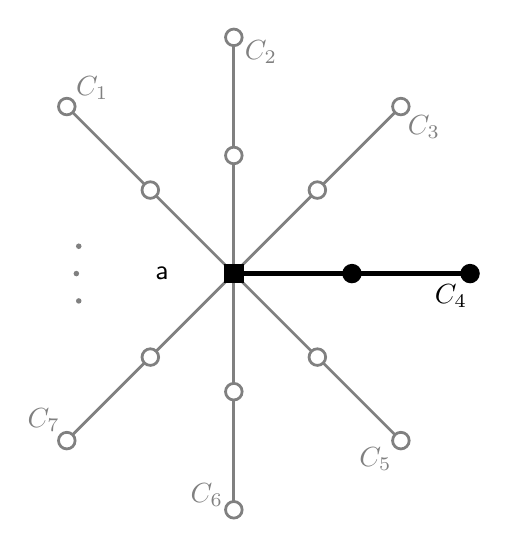
\begin{tikzpicture}
\tikzstyle{every path}=[line width=1pt]
\tikzstyle{every node}=[draw,line width=1pt,inner sep=0]

\tikzstyle{c1}=[rectangle,minimum size=6]

\tikzstyle{d1}=[circle,draw=none,fill,minimum size=2]

\tikzstyle{l7}=[draw=none,circle,minimum size=45]

\draw[gray] (0:0) -- (135:3)
	coordinate[c1,at start] (0)
	coordinate[c1,circle,midway,fill=white] (1)
	coordinate[c1,circle,at end,fill=white,label=35:$C_1$] (2);

\draw[gray] (0.center) -- (90:3)
	coordinate[c1,at start] (0)
	coordinate[c1,circle,midway,fill=white] (3)
	coordinate[c1,circle,at end,fill=white,label=350:$C_2$] (4);

\draw[gray] (0.center) -- (45:3)
	coordinate[c1,at start] (0)
	coordinate[c1,circle,midway,fill=white] (5)
	coordinate[c1,circle,at end,fill=white,label=305:$C_3$] (6);

\draw[gray] (0.center) -- (315:3)
	coordinate[c1,at start] (0)
	coordinate[c1,circle,midway,fill=white] (9)
	coordinate[c1,circle,at end,fill=white,label=215:$C_5$] (10);

\draw[gray] (0.center) -- (270:3)
	coordinate[c1,at start] (0)
	coordinate[c1,circle,midway,fill=white] (11)
	coordinate[c1,circle,at end,fill=white,label=170:$C_6$] (12);

\draw[gray] (0.center) -- (225:3)
	coordinate[c1,at start] (0)
	coordinate[c1,circle,midway,fill=white] (13)
	coordinate[c1,circle,at end,fill=white,label=125:$C_7$] (14);

\draw[black,line width=2pt] (0.center) -- (0:3)
	coordinate[c1,fill,at start] (0)
	coordinate[c1,circle,fill,midway] (7)
	coordinate[c1,circle,fill,at end,label=260:$C_4$] (8);

\coordinate[l7,label=180:${\textsf a}$] (0) at (0.center);

\coordinate[d1,gray] (.) at (190:2);
\coordinate[d1,gray] (.) at (180:2);
\coordinate[d1,gray] (.) at (170:2);
\end{tikzpicture}
\end{center}
\caption{(Color online)
Greechie orthogonality diagram of a star-shaped configuration,
representing a common basis element/projector ${\textsf a}$ with an overlaid two-valued assignment reflecting $v({\textsf a})=1$.
It is assumed that the system is prepared in state $C_4$, depicted by a block colored in thick filled black;
all the other (continuity of) contexts are   ``phantom contexts'' colored in gray.
(Compare also Ref. \cite[Fig.~2]{2012-incomput-proofsCJ}.)
}
\label{2012-psiqm-v2}
\end{figure}



With the  single pure state conjecture,
the Kochen-Specker theorem (although of course remaining correct) does not apply any more,
because one of its implicit assumptions -- (i) the simultaneous co-existence of the observables and contexts involved in the argument --
does not hold any longer.
For the sake of demonstration, consider the rule that, under the Kochen-Specker assumptions, for a configuration
of contexts as depicted in Fig.~\ref{2012-psiqm-v2-f2},
if the state is prepared in context $C_1$, with $v({\textsf a})=1$ (i.e. the detector corresponding to observable ${\textsf a}$ clicks),
this implies $v({\textsf b})=0$; that is, a detector corresponding to observable $b$ will not click.
[A rather simple proof by contradiction (wrongly) assumes that $v({\textsf a})=1$  as well as $v({\textsf b})=1$
can consistetly coexist, thereby leading to a complete contradiction, since in this case
the value assignment of both link observables for $C_3/C_5$ as well as $C_4/C_5$ have to be  1,
alas these link observables belong to the same block $C_5$.]
That quantum mechanics contradicts this prediction  $v({\textsf a})=1-v({\textsf b})=1$ is an immediate consequence of the fact that,
because ${\textsf a}$ and ${\textsf b}$ are not in the same block, ${\textsf a}$ cannot be orthogonal to ${\textsf b}$,
and hence
$\langle {\textsf a} \vert {\textsf b} \rangle \neq 0$, implying a nonvanishing probability $\vert \langle {\textsf a} \vert {\textsf b} \rangle  \vert^2 >0$
[for a concrete though not unique parametrization of the ``bug'' configuration, see
Fig.~4.2 in Ref.~\cite{svozil-tkadlec}, in which
${\textsf a}\equiv \left(\sqrt{2},1,0\right)$
${\textsf b}\equiv \left(\sqrt{2},-1,0\right)$].

However, since according to  the  single pure state conjecture
only $C_1$ exists, any argument based on the simultaneous co-existence of the
non-comeasurable contexts $C_2$--$C_7$ is inapplicable for quantized systems.
\begin{figure}[h]
\begin{center}
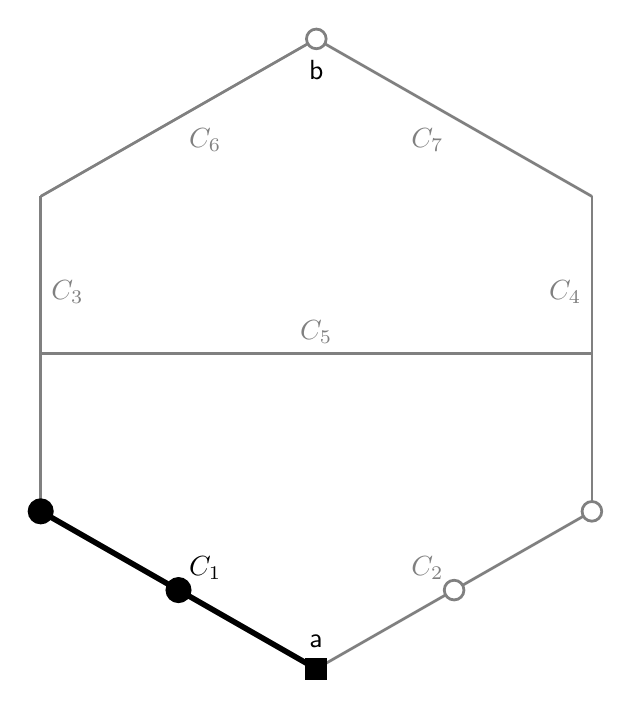
\begin{tikzpicture} [scale=0.5]

\tikzstyle{every path}=[line width=1pt]
\tikzstyle{c1}=[rectangle,minimum size=8]

%\draw[help lines,orange] (-7,-8) grid (7,8);


\draw[gray]  (7,4) -- (7,-4);
\node [above left, gray] at (7,1) {$C_4$};

\draw[gray]  (7,-4) -- (0,-8) ;
\node [above left, gray] at (3.5,-6) {$C_2$};
\draw[gray,fill=white] (7,-4) circle [radius=0.25];
\draw[gray,fill=white] (3.5,-6) circle [radius=0.25];

\draw[gray]  (-7,-4) -- (-7,4);
\node [above right, gray] at (-7,1) {$C_3$};

\draw[gray]  (-7,4) -- (0,8) ;
\node [below right, gray] at (-3.5,6) {$C_6$};

\draw[gray]  (0,8) -- (7,4);
\draw[gray,fill=white] (0,8) circle [radius=0.25];
\node [label=below:${\textsf b}$, gray] at (0,8) {};
\node [below left, gray] at (3.5,6) {$C_7$};


\draw[gray]  (-7,0) -- (7,0);
\node [above, gray] at (0,0) {$C_5$};

\draw [line width=2pt,black]  (0,-8) -- (-7,-4)
	coordinate[c1,circle, at end,fill=black] (0)
	coordinate[c1,circle,midway,fill=black] (1)
	coordinate[c1,rectangle,at start,fill=black] (2);
\node [above right, black] at (-3.5,-6) {$C_1$};
\node [label=above:${\textsf a}$, black] at (0,-8) {};

\end{tikzpicture}
\end{center}
\caption{(Color online)
``Bug-type'' \cite{Specker-priv} Greechie orthogonality diagram
with an overlaid two-valued assignment reflecting ``$v({\textsf a})=1$ implies $v({\textsf b})=0$.''
This configuration is part of the original
proof of the Kochen-Specker theorem \cite[$\Gamma_1$]{kochen1}.
For concrete coordinatizations, see, for instance, the original paper by Kochen and Specker, as well as Ref.~\cite{svozil-tkadlec,2012-incomput-proofsCJ}.
It is assumed that the system is prepared in state $C_1$, depicted by a block colored in thick filled black;
all the other six remaining contexts $C_2$--$C_7$ are   ``phantom contexts'' colored in gray.
}
\label{2012-psiqm-v2-f2}
\end{figure}

\section{Is the best interpretation of the quantum formalism its non-interpretation?}

Finally, let me mention a few thoughts on ``interpretation and meaning.''
Time and again, the quantum theorist is reminded by prestigious peers that the best
interpretation of quantum mechanics appears to be its non-interpretation \cite{Fuchs-Peres}.
Indeed, as has been pointed out earlier, it has become almost fashionable to discredit interpretation
and causality in the quantum domain.
Already Sommerfeld warned his students not to get
into these issues,
and not long ago scientists working in that field
have had a hard time not to appear as ``quacks'' \cite{clauser-talkvie}.

In favour of non-interpretation one could maintain that
interpretation is to the formalism what a
scaffolding in architecture and
building construction is to the completed building.
Very often the scaffolding has to be erected because
it is an indispensable part of the building process.
Once the completed building is in place, the scaffolding is torn down and
the {\em opus} stands in its own full glory.
No need for auxiliary scaffold any longer.

However, it is my conviction
that nobody in quantum mechanics gets along without any interpretation
and intuition.
Indeed, a {\it Haltung} towards non-interpretation of the formalism would inevitably cripple further physical progress.
Because by historic analogy we can suspect that, as time goes by, so will be our physical formalisms \cite{lakatosch},
and that, as has been expressed by Greenberger \cite{greenberger-talk-99}, four hundred years from now
all our present physical theories will appear ``laughable.''

Yet we are confronted with a situation in which an orthodoxy tries to suppress and avoid thinking about the ``how'' \cite[p.~129]{feynman-law},
or at least advises ``not worry too much''  \cite{dirac-noworries},
while at the same time expressing the opinion that certain events occur {\it ex nihilo} (out of nothing), fundamentally
inexplicably, and irreducibly random \cite{zeil-05_nature_ofQuantum}.
This, I believe, is tantamount to dogmatism,
and contradictory to all rationalistic principles on which scientific progress thrives.

It is my conviction that
without interpretations, the application of the formalism would be restricted to
automatic proofing, to an ``a thousand monkeys typing-away scenario.''
Quantum mechanics would become another application of (rather elementary) linear algebra.
Hence   there will be no significant scientific progress in this area without
attempts to give meaning to what is formalized.
Therefore, interpretation should not be discredited,
but considered wisely with {\em evenly-suspended attention}
\cite{Freud-1912}.

\section{Consequences for quantum random number generators}

Let me finally discuss the situation with regard to certain practical implementations of quantum random number generators.
Although, as has been mentioned earlier,
quantum randomness, or at least Turing incomputability from quantum coin tosses involving beam splitters,
is often judged to be the ``ultimate'' randomness,
and even ``the (nihilistic) message of the quantum,''
some questions with regard to the conceptual foundations arise.
For instance, an ideal beam splitter can be modelled by a unitary transformation,
which is a (Laplacian type causal) one-to-one isometric transformation in Hilbert space.

No information is lost in such devices, which are (at least ideally) incapable of irreversibility.
Operationally this can be demonstrated by the serial composition of two beam splitters,
which effectively renders a Mach-Zehnder interferometer yielding the original quantum state in its output ports.

One may speculate that the ``randomness resides'' in the (classical) detection of,
say, the photons, after the half-silvered mirror.
But, as has for instance been pointed out by Everett, this is (self-)delusional,
as quantum mechanics,
and in particular the unitary quantum evolution of all components involved in the detection,
at least in principle,
must hold uniformly.

The  situation discussed is also related to the issue of  ``quantum jellification''
posed by the late Schr\"odinger with regards to the coherent superposition
and co-existence of classically contradictory physical states.
But how can irreversibility possibly ``emerge'' from reversibility?
Besides "for-all-practical-purposes" being effectively irreversible,
in principle there does not seem to exist any conceivable unitary route to irreversibility;
at least if quantum theory is universally valid.

We have therefore posed two simple questions; one formal and one empirical:
the formal one is about the (im)possible ``emergence'' of noninvertible mappings from invertible ones;
the empirical question is about the (non-)existence of principal bounds on reconstructing a state after ``measurement.''

Because, in view of a causal, bijective Laplacian type quantum evolution, what guarantees a quantum coin toss, say,
on a half-silvered mirror, to perform irreducibly random,
and where exactly does this randomness originate?
The issues appear as marred today as in Everett's and Wigner's times \cite{wigner:mb},
but they are much more pressing now, as the associated technologies \cite{zeilinger:qct,stefanov-2000}
have been deployed for experiments \cite{wjswz-98}
as well as cryptanalysis and industry by various spin-offs.



One possibility to circumvent this conundrum is by postulating that
(i) at every instant, only a single state (or context) exists;
and that
(ii)
through {\em context translation,}
in which a mismatch between the preparation and the measurement results in the ``translation''
of the original information encoded by a quantum system into the answer requested,
noise is introduced by the many degrees of freedom of a suitable ``quasi-classical'' measurement apparatus.
This would be an altogether different source of randomness than an
irreducible creation of information {\it ex nihilo} (``out of nothing'')
that is favoured by the present quantum orthodoxy.

\begin{acknowledgements}
 This research has been partly supported by FP7-PEOPLE-2010-IRSES-269151-RANPHYS.
This contribution was done in part during a visiting honorary appointment at the University of Auckland, New Zealand.
Discussions during a {\em LARSIM/QuPa workshop on physics and computation} at the {\it Institut Henri Poincar\'e}, Paris on June 28-29, 2012,
where a previous version of this paper has been presented, are gratefully acknowledged.
I gratefully acknowledge the help and explanations of Professor Constantine Tsinakis with respect to group theory, and other algebraic issues.
\end{acknowledgements}

 \bibliography{svozil}

\end{document}


~~~~~~~~~~~~~~~~~~~~~~~~~~~~~~~~~~~~~~



Normalize[z_]:= z/Sqrt[z.Conjugate[z]];

(* Definition of the Tensor Product *)
TensorProduct[a_, b_] :=
  Table[(*a,b are nxn and mxm-matrices*)
   a[[Ceiling[s/Length[b]], Ceiling[t/Length[b]]]]*
    b[[s - Floor[(s - 1)/Length[b]]*Length[b],
      t - Floor[(t - 1)/Length[b]]*Length[b]]], {s, 1,
    Length[a]*Length[b]}, {t, 1, Length[a]*Length[b]}];


(* Definition of the Tensor Product between two vectors *)

TensorProductVec[x_, y_] :=
  Flatten[Table[
    x[[i]] y[[j]], {i, 1, Length[x]}, {j, 1, Length[y]}]];


(* Definition of the Dyadic Product *)

DyadicProductVec[x_] :=
  Table[x[[i]] Conjugate[x[[j]]], {i, 1, Length[x]}, {j, 1,
    Length[x]}];

DyadicProduct2Vec[x_,y_] :=
  Table[x[[i]] Conjugate[y[[j]]], {i, 1, Length[x]}, {j, 1,
    Length[y]}];


(* Definition of some bases *)

BellBasis = (1/Sqrt[2]) {{1, 0, 0, 1}, {0, 1, 1, 0}, {0, 1, -1,
     0}, {1, 0, 0, -1}};

CartesianBasis4Dim = {{1, 0, 0, 0}, {0, 1, 0, 0}, {0, 0, 1, 0}, {0, 0, 0, 1}};


CartesianBasisNDim[N_] := Table[ Table[ KroneckerDelta [i,j]
                                       ,{j, 1, N}]
                                ,{i, 1, N}];

UnitaryOperatorFromBases[a_,b_] :=  Sum[ DyadicProduct2Vec[ a[[i]],b[[i]] ] , {i, 1,
    Length[a]}];

UnitaryOperatorFromBases[CartesianBasisNDim[4],
   BellBasis].UnitaryOperatorFromBases[CartesianBasisNDim[4],
   BellBasis] \[HermitianConjugate]


ShiftPermutedBasis[a_] := Delete[Append[ a, a[[1]] ] , 1 ];

ShiftPermutedBasis[CartesianBasisNDim[3]]


V =  UnitaryOperatorFromBases[CartesianBasisNDim[3],ShiftPermutedBasis[CartesianBasisNDim[3]]]

V.V\[HermitianConjugate] == IdentityMatrix[3]

FullSimplify[{Normalize[FullSimplify[Eigenvectors[V][[1]]]],Normalize[FullSimplify[Eigenvectors[V][[2]]]],Normalize[FullSimplify[Eigenvectors[V][[3]]]]}]

V.(V.V) == IdentityMatrix[3]

Simplify[ComplexExpand[E^(2 Pi I/3)] /Sqrt[3]]

Simplify[ComplexExpand[E^(4 Pi I/3)] /Sqrt[3]]


V1 =  UnitaryOperatorFromBases[CartesianBasisNDim[3],ShiftPermutedBasis[ShiftPermutedBasis[ShiftPermutedBasis[CartesianBasisNDim[3]]]]]

V1.V1\[HermitianConjugate] == IdentityMatrix[3]

FullSimplify[{Normalize[FullSimplify[Eigenvectors[V1][[1]]]],Normalize[FullSimplify[Eigenvectors[V1][[2]]]],Normalize[FullSimplify[Eigenvectors[V1][[3]]]]}]

V1.(V1.V1) == IdentityMatrix[3]


~~~~~~~~~~~~~~~~~~~~~~~~~~~~~~~~~~~~~~~~~~~~~~~~~~~~

V = UnitaryOperatorFromBases[BellBasis,
  ShiftPermutedBasis[ShiftPermutedBasis[BellBasis]]]

FullSimplify[{Normalize[FullSimplify[Eigenvectors[V][[1]]]],
  Normalize[FullSimplify[Eigenvectors[V][[2]]]],
  Normalize[FullSimplify[Eigenvectors[V][[3]]]],
  Normalize[FullSimplify[Eigenvectors[V][[4]]]]}]

MatrixForm[%]
